Negli ultimi anni, la grande presenza di dipositivi in grado di catturare la posizione di un oggetto nel
tempo e le sue variazioni hanno prodotto enormi quantità di dati.
L'analisi di questi dati, resa possibile dalle moderne tecnologie Big Data, apre molteplici possibilità, come
ad esempio la ricerca dei flussi di traffico all'interno di un terriorio cittadino, oppure l'individuazione
dei luoghi più visitati da una certa categoria di utenti, o ancora il riconoscimento di gruppi di oggetti che si
muovono assieme all'interno di un certo spazio e tempo.
Dato il grande numero di potenziali fonti per i dati, è necessario ricondurre questi ultimi a una formulazione comune
così da poter sfruttare al meglio le loro potenzialità espressive.
La rappresentazione più basilare consiste nel considerare una traiettoria come l'insieme delle posizioni
spaziali dei punti che la compongono associando a ciascuno l'istante temporale in cui è stato registrato.
Questa formulazione prende il nome di traiettoria grezza \textit{raw trajectory}, vedi~\cref{fig:chap-1:trajectory}
Andando a formalizzare quanto detto sopra:

\begin{figure}
  \centering
  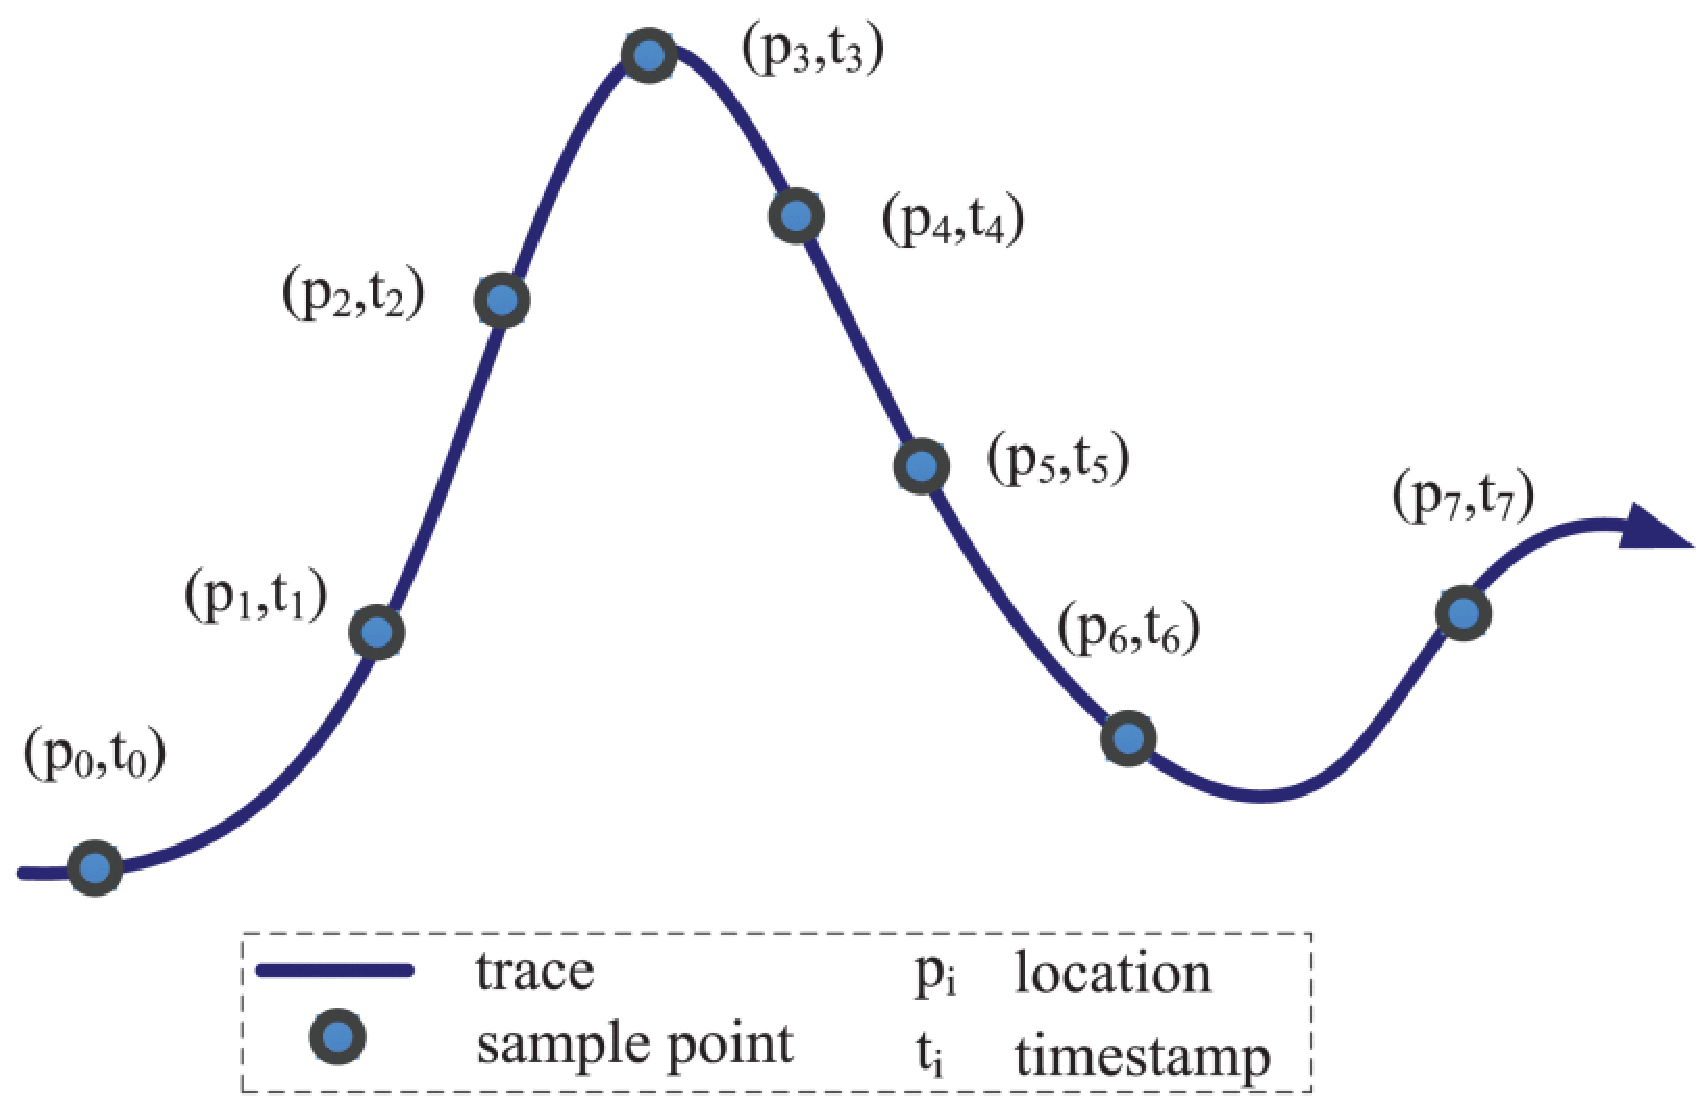
\includegraphics[scale=.5]{/sec-1/trajectory.pdf}
  \caption{Esempio di traiettoria,Fonte:\url{https://www.semanticscholar.org/paper/A-Survey-on-Trajectory-Data-Mining\%3A-Techniques-and-Feng-Zhu/a32f521442a540a6d1420526eaa68b3cab6b1d0d}}%
  \label{fig:chap-1:trajectory}
\end{figure}

\begin{definition}[Traiettoria]

  Si definisce una traiettoria grezza, o \textit{raw trajectory}, una sequenza temporale di punti \({p_{t}, p_{t'},\ldots, p_{t''}}\)
  tale che ogni punto \(p_{t}\) è composto da una coppia di coordinate spaziali \((latitude, longitude)\) e un tempo\(t\).

\end{definition}

Questa basilare e semplice modalità di espressione può essere successivamente complicata, ad esempio adottando
una scala unica tra le diverse traiettorie per lo spazio e una per il tempo, oppure aggiungendo ulteriori informazioni, come ad esempio la direzione o attributi
dell'oggetto che la genera.

Per aumentare l'espressività della singola traiettoria, può essere utile definire il concetto di sotto-traiettoria, o \textit{subtrajectory}.
Intuitivamente una sotto-traiettoria non è altro che un segmento di una traiettoria relativo a un certo sottoinsieme dello spaziotempo coperto da quest'ultima.

\begin{definition}[Sottotraiettoria]

  Date due traiettorie \(TR\textsubscript{i}, TR\textsubscript{j}\) si definisce  \(TR\textsubscript{i}\) sottotraiettoria di \(TR\textsubscript{j}\) se \(\forall p_{t\textsubscript{i}} \in TR\textsubscript{i}, p_{t\textsubscript{i}} \in TR\textsubscript{j}\).

\end{definition}


